\documentclass[conference]{IEEEtran}
\IEEEoverridecommandlockouts
% The preceding line is only needed to identify funding in the first footnote. If that is unneeded, please comment it out.
\usepackage{cite}
\usepackage{amsmath,amssymb,amsfonts}
\usepackage{algorithmic}
\usepackage{graphicx}
\usepackage{textcomp}
\usepackage{xcolor}
\usepackage{subfigure}
\usepackage{makecell}
\usepackage[T1]{fontenc}
\def\BibTeX{{\rm B\kern-.05em{\sc i\kern-.025em b}\kern-.08em
    T\kern-.1667em\lower.7ex\hbox{E}\kern-.125emX}}
\begin{document}
\title{Numerical simulation of cancer cells electroporation based on mesh transport network method
\thanks{This work was supported in part by the Science and Technology Research Program of Chongqing Municipal Education Commission (Grant No.KJQN202100607), in part by the Natural Science Foundation of China (No. 51507024).}
}
\author{
\IEEEauthorblockN{1\textsuperscript{st} Fei Guo}
\IEEEauthorblockA{\textit{Institute of Ecological Safety} \\
\textit{Chongqing University of Posts and Telecommunications}\\
Chongqing, China\\
guofei@cqupt.edu.cn}
\and
\IEEEauthorblockN{2\textsuperscript{nd} Yapeng Zhang}
\IEEEauthorblockA{\textit{Institute of Ecological Safety} \\
\textit{Chongqing University of Posts and Telecommunications}\\
Chongqing, China\\
s210331153@stu.cqupt.edu.cn}
\and
\IEEEauthorblockN{3\textsuperscript{rd} Jiaguo Sun}
\IEEEauthorblockA{\textit{Institute of Ecological Safety} \\
\textit{Chongqing University of Posts and Telecommunications}\\
Chongqing, China\\
s210331093@stu.cqupt.edu.cn}
\and
\IEEEauthorblockN{4\textsuperscript{th} Xinghe Gou}
\IEEEauthorblockA{\textit{Institute of Ecological Safety} \\
\textit{Chongqing University of Posts and Telecommunications}\\
Chongqing, China\\
s220303005@stu.cqupt.edu.cn}
}
\maketitle

\begin{abstract}
The use of large pulsed electric fields to induce electroporation (EP) is a technique that can significantly alter the biological permeability of cell membranes and can be used to ablate tumor tissue and kill cancer cells. In this study, based on mesh transport network method (MTNM), we calculated the asymptotic EP model with the cancer cell anode perpendicular and parallel to the electric field direction. The results indicate that the density and rate of generation of pores at the recessed sites of the cancer cell membrane are dramatically reduced. In addition, the perforation time and the arc length ratio (ALR) of cancer cells changes when they are exposed to an electric field with different electric field directions. In our simulations, when the cell anode was perpendicular to the direction of the electric field, the ALR at the site of the depressed membrane of the cancer cells was 16.7\% higher than the ALR at the raised site of the membrane. This work can provide guidance for the selection of parameters for the cancer cell EP process.
\end{abstract}

\begin{IEEEkeywords}
electroporation, cancer cell, numerical simulation, MTNM
\end{IEEEkeywords}

\section{Introduction}
Electroporation (EP) is a phenomenon in which the lipid bilayer of a cell membrane is rearranged to form aqueous pores in response to stimulation by large electric field, thereby altering the permeability of the cell membrane\cite{kotnik2019membrane}. EP can be categorized as conventional EP, which uses long duration, small magnitude pulses to induce small, recoverable pores in the cell plasma membrane only, and supra-EP, which uses short duration, large magnitude pulses to cause significant EP and induce large, non-recoverable pores in plasma and organelle membranes. Conventional EP can be used for plasmid transfection and drug delivery\cite{b3,a2010electroporation}. Supra-EP significantly increases cell permeability and even induces apoptosis, in the fields of tumour tissue ablation and food processing, it has become an effective tool.

However, the lack of understanding of the basic mechanism of EP has to some extent hindered the application and development of EP in medicine\cite{yarmush2014electroporation}, biology\cite{cao2019nontoxic} and food industry\cite{golberg2010use}. On the one hand, there are a large number of studies on EP mechanisms based on pulse parameters, tissues and pore populations, but none of them is able to thoroughly explain the mechanisms of the EP phenomenon\cite{rebervsek2011advantages,smith2014emergence}. On the other hand, the EP studies of cells have mainly focused on normal cells, but EP of cancer cells with irregular shapes has not been studied in sufficient depth. The shape of the cell membrane of cancer cells is different from that of normal cells, and the EP pattern of normal cells cannot be perfectly adapted to cancer cells. Therefore, it is very significant to establish a numerical model EP of cancer cells. Our work can provide useful guidance for therapeutic protocol for the tumour ablation and cancer cell killing.

\section{Method}
\subsection{Model System}
In our simulation, each cancer cell is assumed to have homogeneous (core-shell structures two-dimensional modeling biological cells) phospholipid bilayer membrane of 5 nm thickness. The cancer cell in A and B were described using the Gielis'~superformula\cite{mescia2017modeling}, as followed:
\begin{subequations}
	\begin{equation}
		x=-k_x R(\theta)sin(\theta)
	\end{equation}
	\begin{equation}
		y=k_y R(\theta)cos(\theta)
	\end{equation}
	\begin{equation}
		R(\theta)=\left(\left| \frac{cos(m_1\theta/4)}{a_1} \right|^{n_1}+\left|\frac{sin(m_2\theta/4)}{a_2}\right|^{n_2}\right)^{-\frac{1}{b_1}}
	\end{equation}
\end{subequations}
and 
\begin{subequations}
	\begin{equation}
		x=k_x R(\theta)cos(\theta)
	\end{equation}
	\begin{equation}
		y=k_y R(\theta)sin(\theta)
	\end{equation}
	\begin{equation}
		R(\theta)=\left(\left| \frac{cos(m_1\theta/4)}{a_1} \right|^{n_1}+\left|\frac{sin(m_2\theta/4)}{a_2}\right|^{n_2}\right)^{-\frac{1}{b_1}}
	\end{equation}
\end{subequations}
where $\theta\in\lbrack 0~2\pi \rbrack$ is a angle parameters. Superformula parameters $k_x=k_y=16.8~\mu m$, $m_1=m_2=6$, $n_1=n_2=1$, $a_1=a_2=1$ and $b_1=-2$. The cancer cells in B are identical to those in A. To study the effect of different electric field orientations on the EP results of the cancer cells, the cancer cell in B are rotated by $90^\circ$, as shown in Fig.\ref{fig::1a} and Fig.\ref{fig::1b}. The cancer cell model is an approximation of MCF--7 breast cancer cells\cite{medlock2017cancer}. The bounding box for the system is $200~\mu m \times 200 ~\mu m$, with the cell centered.
\begin{figure}[htbp]
	\centering
	\subfigure{
		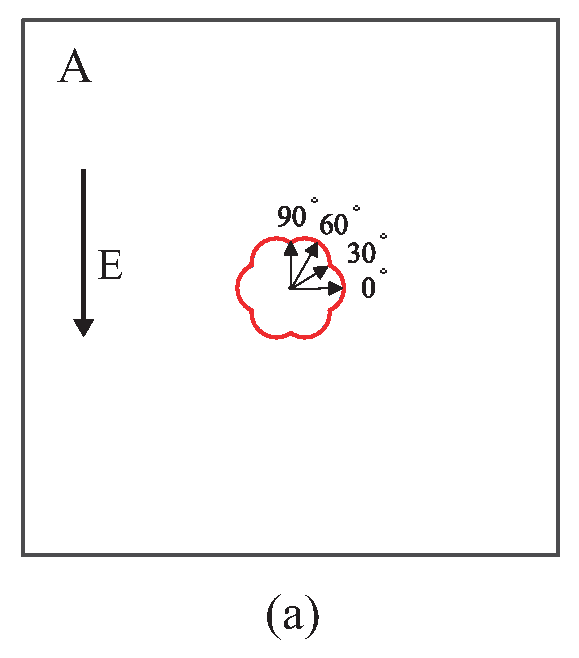
\includegraphics[width=0.2\textwidth]{fig/fig_1a.eps}
		\label{fig::1a}
	}
	\subfigure{
		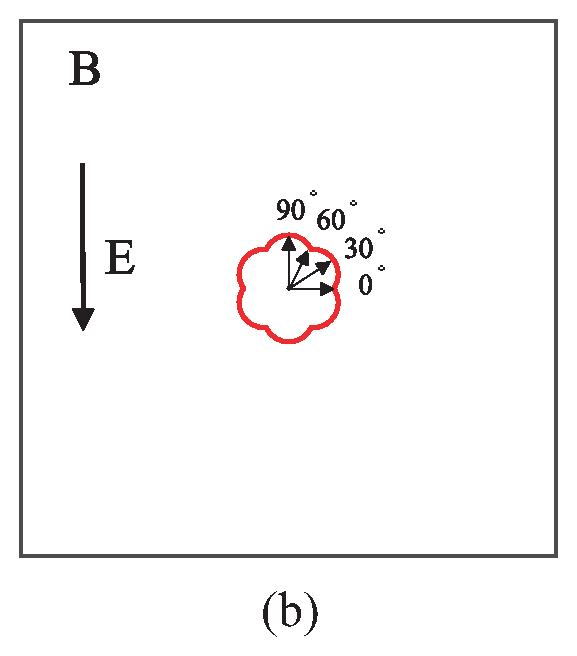
\includegraphics[width=0.2\textwidth]{fig/fig_1b.eps}
		\label{fig::1b}
	}
	\caption{Cell system model geometry and electric field pulse. (a), (b) Cancer cell A and B are described by the	Gielis’ superformula, the shortest cell radius $R_{min} = 16.8\mu m$ , and the longest cell radius $R_{max} = 19.98\mu m$.}
	\label{fig::1}
\end{figure}

To study irreversible electroporation (IRE) in cancer cells, an ideal trapezoidal nanosecond pulse, with an electric field strength of $E_{app} = 10~kV/cm$, 10 ns rise--time and 10 ns fall--time, and an 80 ns plateau, was applied to the upper boundary (anode) and lower (cathode) boundary of the cell system bounding box in parallel, the total simulation runtime is 200 ns. The electrical parameters of the cell system are described in Ref\cite{mescia2017modeling, smith2006modeling}. 
\subsection{Meshed Transport Network Method}
Triangular meshes of the cell system were generated using an open source algorithm. The algorithm produces high quality meshes with elements that may vary widely in size. The Meshed transport network method (MTNM) is an improvement of the transport lattice method (TLM) model\cite{gowrishankar2003approach, stewart2004transport}. This model establishes equivalent circuits between discrete nodes and uses the asymptotic model of EP to calculate the creation process of pores on the plasma membrane. Fig.\ref{fig::2a} shows the electrical transport between adjacent VCs $j$ and $k$. There exists an electric field $\vec{E}_{j,k}$ and current density $\vec{J}_{j,k}$ at the interface of VCs $j$ and $k$. There vectors may be separated into components normal and parallel to the interface, and clearly only the former contribute to transport between the VCs. The difference in potential between VCs $j$ and $k$ is $\left ( \Delta \phi  \right ) _{j,k}=\phi _k-\phi_j$, a share interface of area $w_{j,k}d$, a nodal separation $l_{j,k}$ and contain a medium with conductivity $\sigma$ and permittivity $\epsilon$. Thus, the total current flowing from VC $j$ to VC $k$ is 
	\begin{equation}
	\begin{split}
		i_{j,k} &= w_{j,k}(\vec{J}^{j,k}_{\bot }\cdot \hat{n}_{j,k})\\
		&= w_{j,k}d(\sigma \vec{E}^{j,k}_{\bot} + \epsilon \frac{d}{dt}\vec{E}^{j,k}_{\bot })\\
		&= -w_{j,k}d(\sigma \frac{(\Delta \phi)_{j,k}}{l_{j,k}} + \epsilon \frac{d}{dt} \frac{(\Delta \phi)_{j,k}}{l_{j,k}})\\
		&= -\frac{\left ( \Delta \phi  \right )_{j,k}}{R_{j,k}} - C_{j,k} \frac{d}{dt}\left ( \Delta \phi  \right )_{j,k}   
	\end{split}
	\end{equation}
where $R_{j,k}\equiv l_{j,k}/(\sigma w_{j,k}d)$ and $C_{j,k}\equiv \epsilon w_{j,k}d/l_{j,k}$ and $\vec{E}^{j,k}_\bot = -(\Delta \phi)_{j,k}/l_{j,k}$ is used as the first--order approximation to the normal electric field at the interface. Therefore, the transport between VCs $j$ and $k$ may be represented by a parallel resistor--capacitor pair between nodes $j$ and $k$ may be represented by a parallel resistor--capacitor pair between nodes $j$ and $k$ in the circuit representation of the system. According to Kirchhoff's Current Law, the total current flow out of Voronoi cell $i$ equal zero,
\begin{equation}
	\sum_{k=1}^{N_j}i^{j,k} = 0
\end{equation}

\begin{figure}[htbp]
	\centering
	\subfigure{
		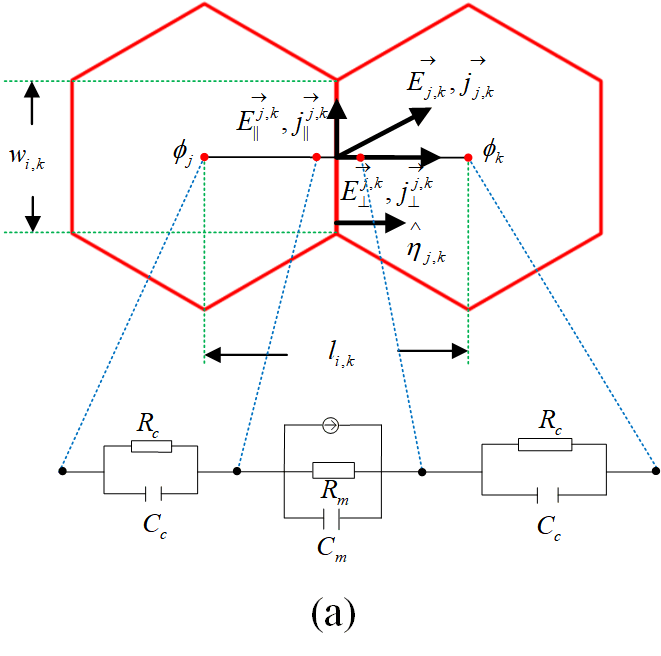
\includegraphics[width=0.3\textwidth]{fig/fig_2a.png}
		\label{fig::2a}
	}
\\
	\subfigure{
		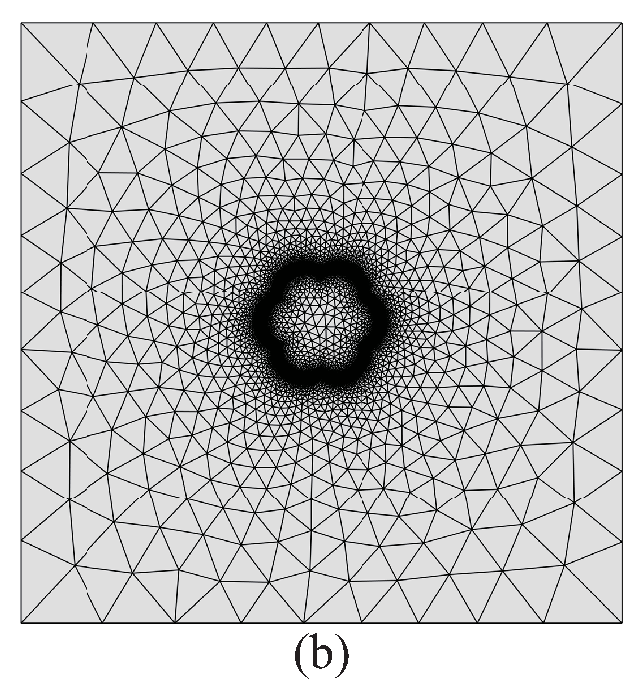
\includegraphics[width=0.2\textwidth]{fig/fig_2b.eps}
		\label{fig::2b}
	}
	\subfigure{
		\includegraphics[width=0.2\textwidth]{fig/fig_2c.eps}
		\label{fig::2c}
	}
	\caption{(a) The equivalent circuit component in the transport network. (b), (c) The Delaunay triangulation generated from the open--source MATLAB mesh generator.}
	\label{fig::2}
\end{figure}

The $200\times200~\mu m$ computational domain is meshed by the MATLAB2021b, and the meshed network of A and B are shown in Fig.\ref{fig::2b} and Fig.\ref{fig::2c}. The computational domains of the two models were meshed as delaunay triangles connected by 7634 nodes (A) and 7332 nodes (B), respectively.
\subsection{Electroporation Model}
 The dynamics of EP often are described by using the Smoluchowski equation with pore creation and destruction rates. In the limit of the pore creation/destruction dominating pore expansion/contraction\cite{powell1986transient}, the Smoluchowski equation simplifies to the ordinary differential equation
\begin{equation}
	\frac{\mathrm{d}N(t)}{\mathrm{d}t} = \alpha e^{\left ( \frac{V_m}{V_{ep}}  \right )^{2}  } \left ( 1-\frac{N(t)}{N_0}e^{-q\left (\frac{V_m}{V_{ep}}   \right )^{2}  }  \right )
\end{equation}
where $N$ is the local pore density, $\alpha$ is the pore creation rate coefficient, $V_m$ is the transmembrane voltage, $V_{ep}$ is the characteristic EP voltage, $N_0$ is the equilibrium pore density for $V_m = 0~V$, and $q$ is an EP coefficient.
\begin{figure}[htbp]
	\centering
	\subfigure{
		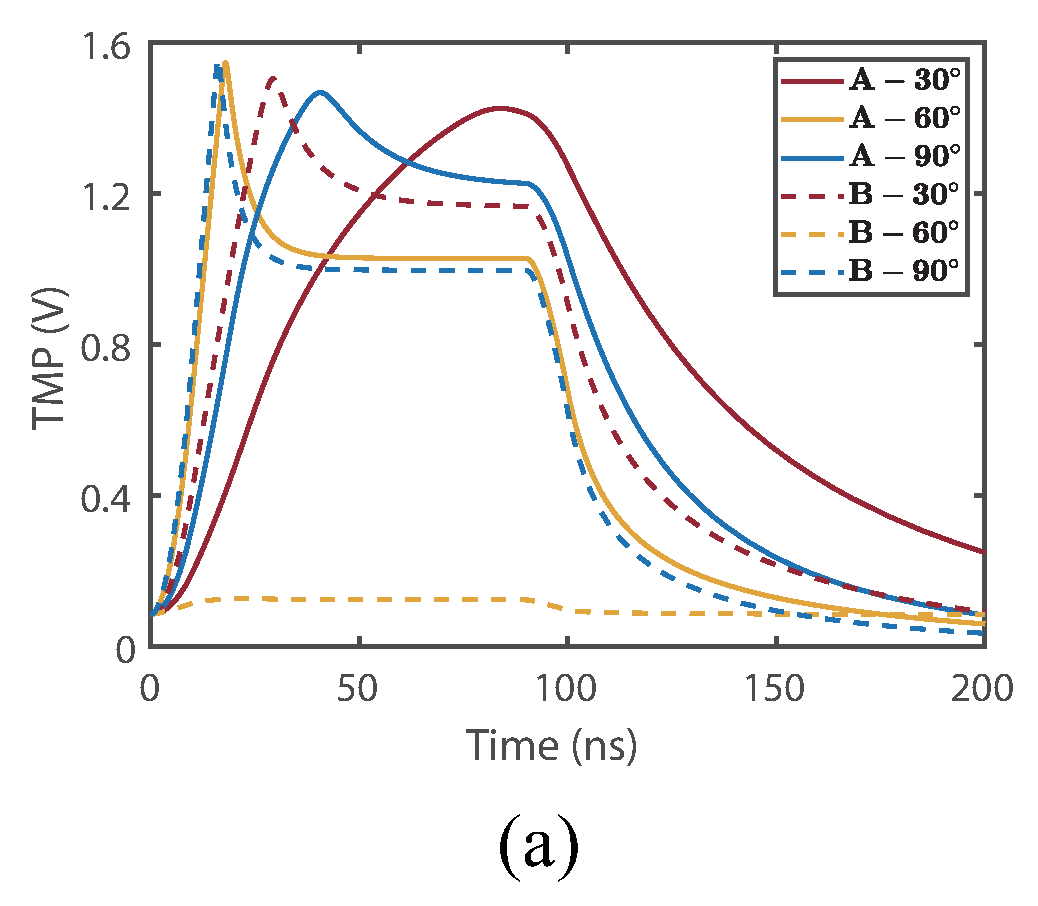
\includegraphics[width=0.21\textwidth]{fig/fig_3a.eps}
		\label{fig::3a}
	}
	\subfigure{
		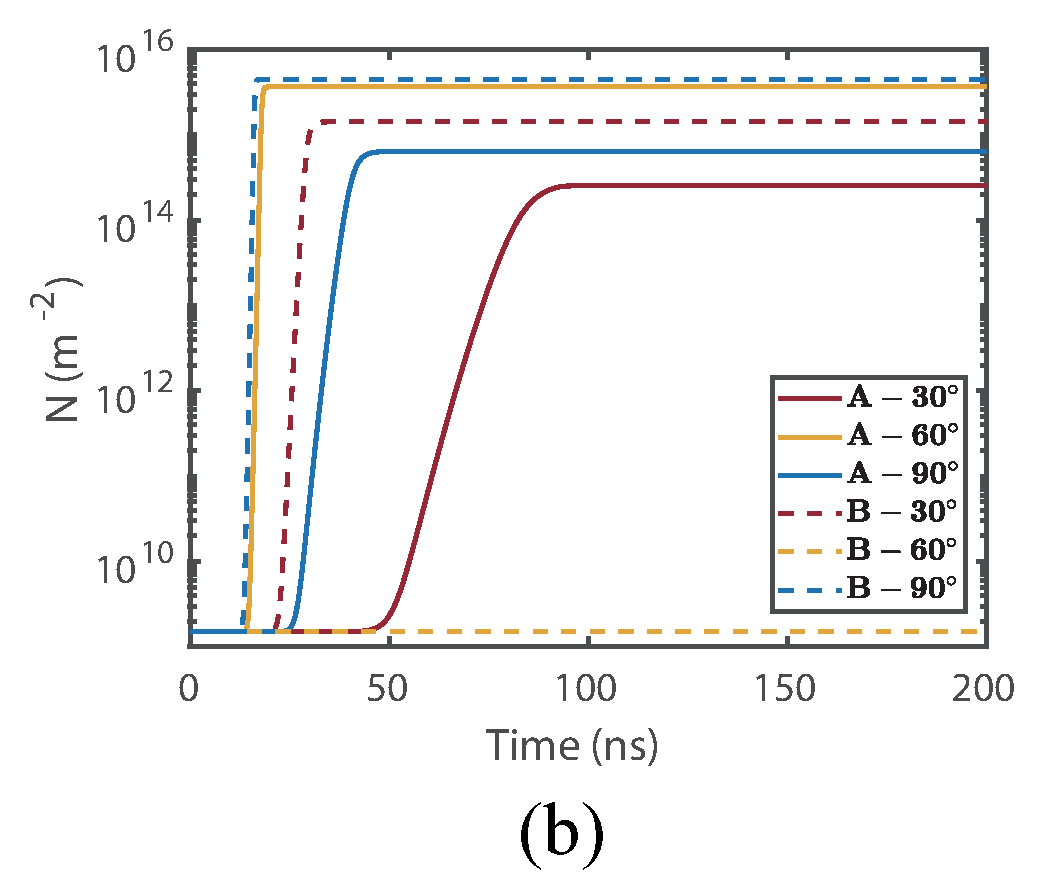
\includegraphics[width=0.21\textwidth]{fig/fig_3b.eps}
		\label{fig::3b}
	}
	
	\caption{(a) Time evolution of the TMP of cancer cells A and B. (b) Time evolution of the pore density of cancer cells A and B.}
	\label{fig::3}
\end{figure}
\section{Result}
The transmembrane potential (TMP) of the cells started to increase after the pulse, and the TMP in the membrane region of cell A and cell B decreased after reaching the EP threshold of \textasciitilde1 V at different times\cite{smith2008active}, as shown in Fig.\ref{fig::3a}. The surge of pores on the membrane directly changes the membrane conductance, so the increase in membrane conductance interrupts the rising process of TMP. $A-60^{\circ}$ reached the TMP peak of 1.548 V at 18.20 ns, but the TMP of $B-60^{\circ}$ increased slowly to 0.128 V \begin{figure*}[htbp]
	\centering
	\subfigure{
		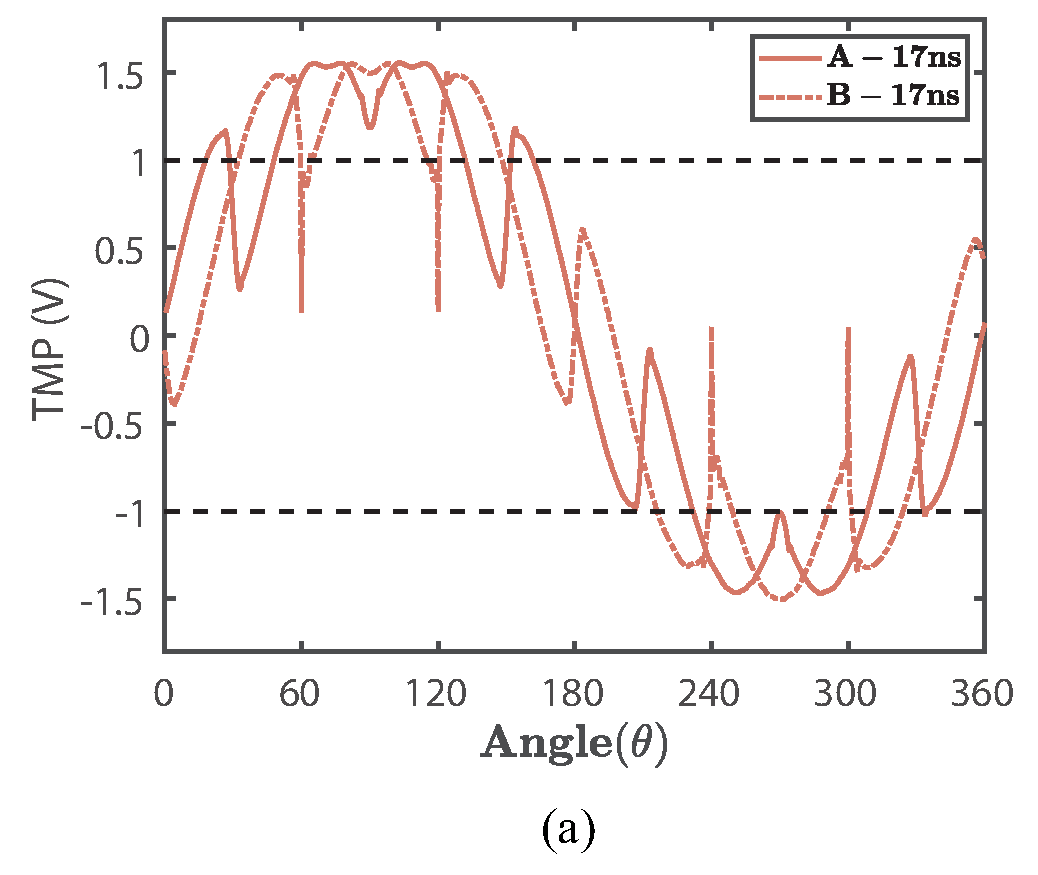
\includegraphics[width=0.25\textwidth]{fig/fig_4a.eps}
		\label{fig::4a}
	}
	\subfigure{
		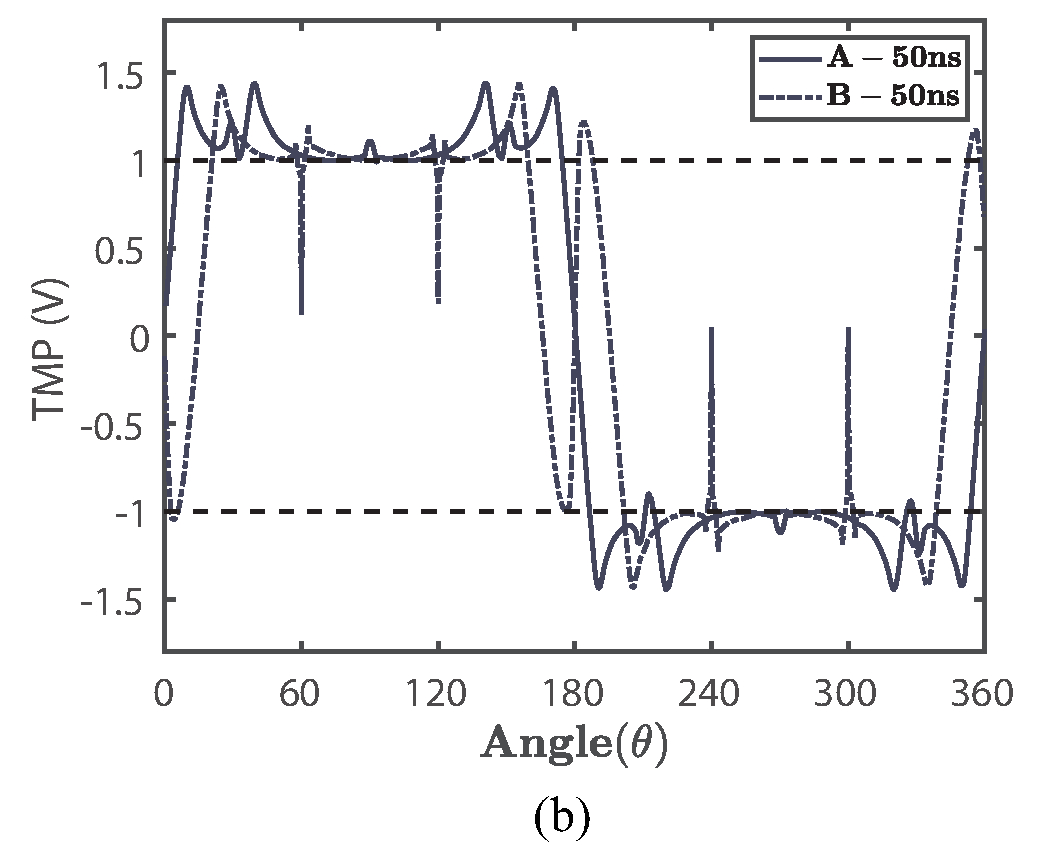
\includegraphics[width=0.25\textwidth]{fig/fig_4b.eps}
		\label{fig::4b}
	}
	\subfigure{
		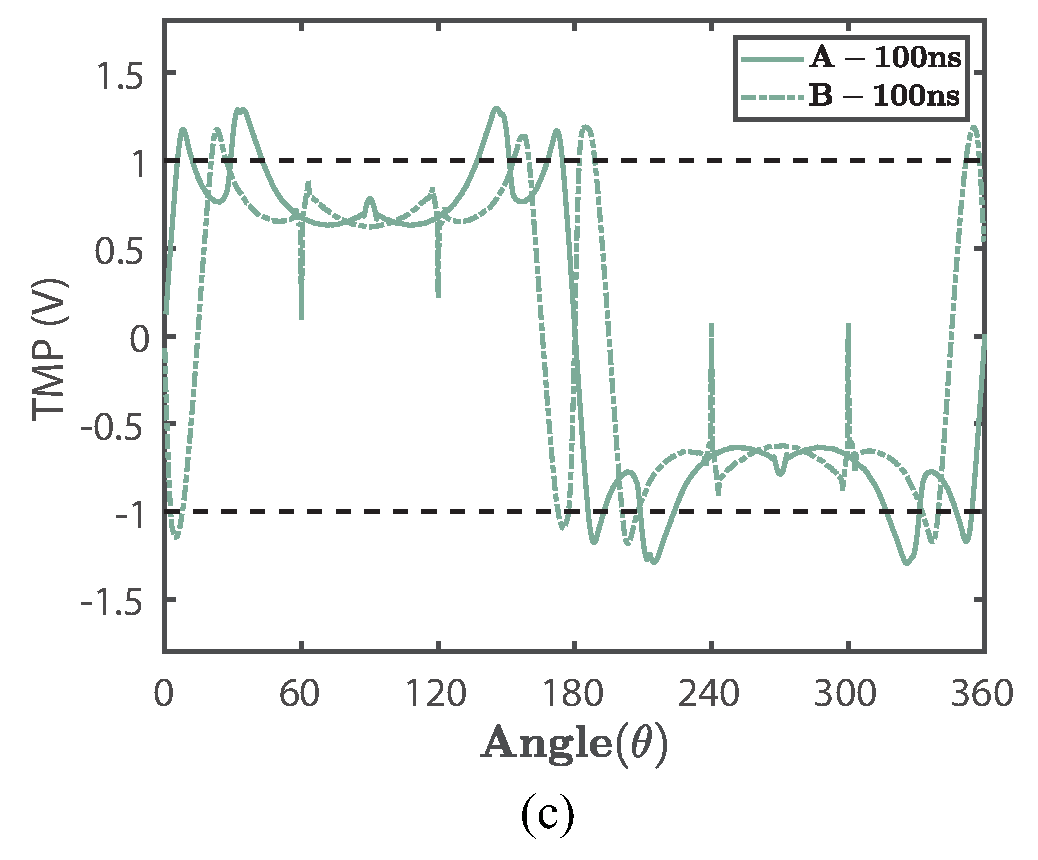
\includegraphics[width=0.25\textwidth]{fig/fig_4c.eps}
		\label{fig::4c}
	}
	
	\caption{Spatial distribution of TMP in cells A and B at 17 ns (a), 50 ns (b), and 100 ns (c).}
	\label{fig::4}
\end{figure*}
\begin{figure*}[htbp]
	\centering
	\subfigure{
		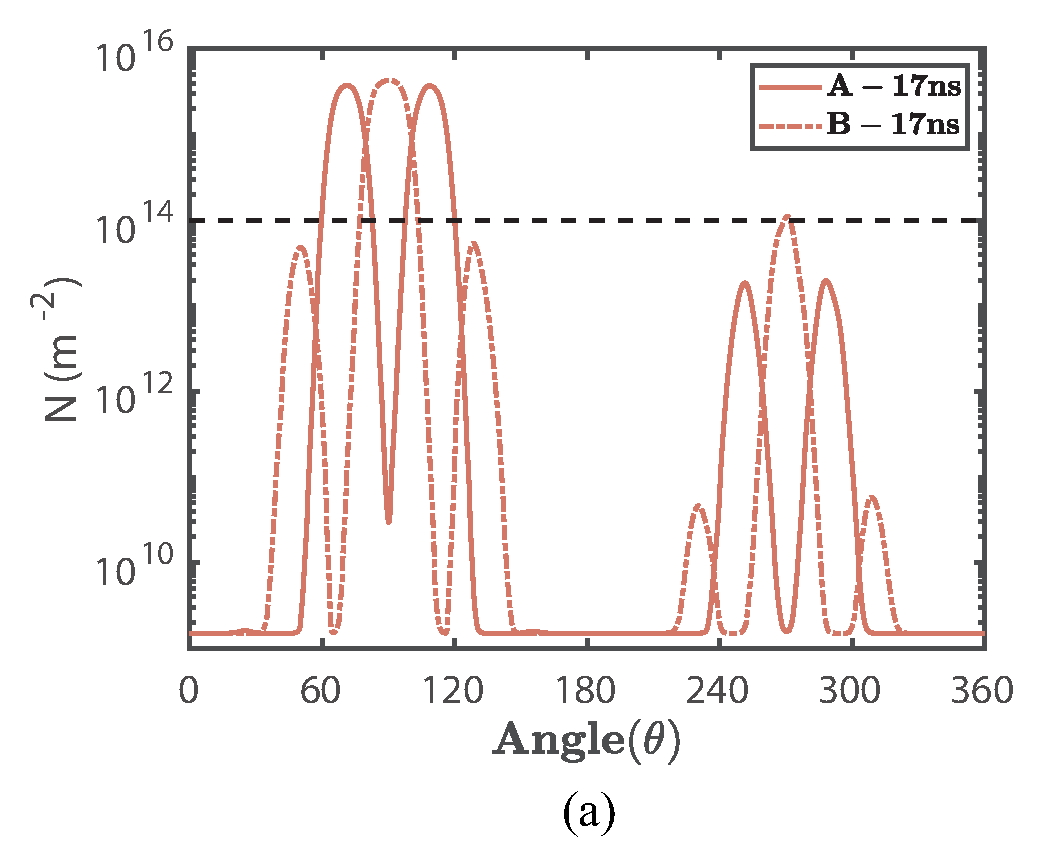
\includegraphics[width=0.25\textwidth]{fig/fig_5a.eps}
		\label{fig::5a}
	}
	\subfigure{
		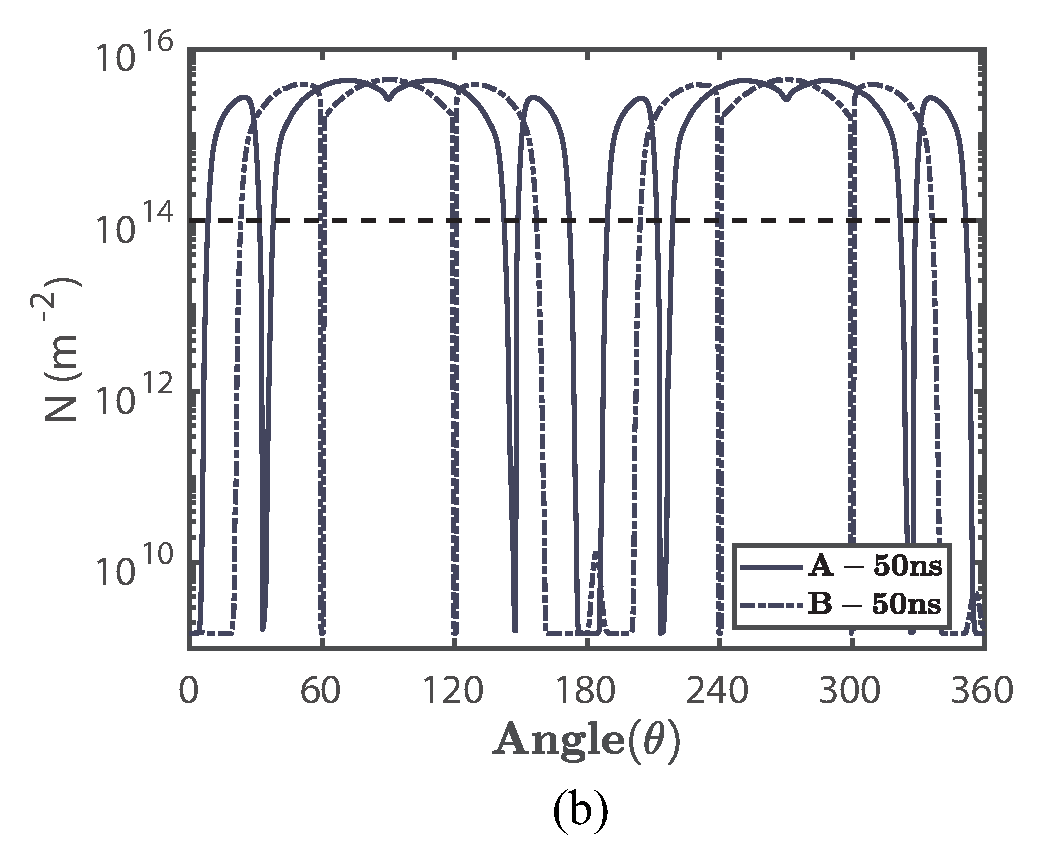
\includegraphics[width=0.25\textwidth]{fig/fig_5b.eps}
		\label{fig::5b}
	}
	\subfigure{
		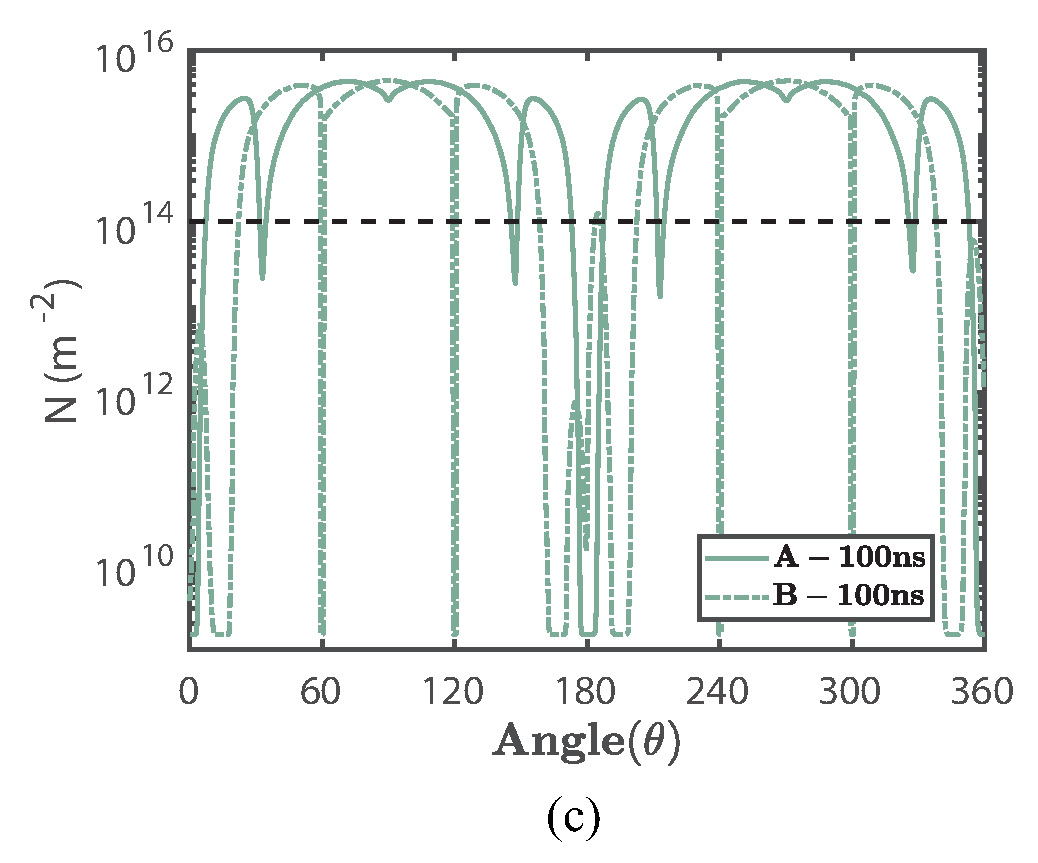
\includegraphics[width=0.25\textwidth]{fig/fig_5c.eps}
		\label{fig::5c}
	}
	\label{fig::5}
	\caption{Spatial distribution of pore density of cells A and B at 17 ns (a), 50 ns (b), and 100 ns (c).}
\end{figure*} at 19.56 ns and continued until the end of the pulse. Cell $A-90^{\circ}$ reached the TMP peak of 1.468 V at 40.71 ns and $B-90^{\circ}$ reached the TMP peak of 1.557 V at 16.19 ns. The TMP peak of cell $B-90^{\circ}$ was 6.1$\%$ higher than that of $A-90^{\circ}$ and the peak time was 24.52 ns earlier. The TMP of $B-60^{\circ}$ did not reach the EP threshold and there was no significant increase in pore space on the membrane, and its pore density remained essentially constant at equilibrium pore density at $V_m=0~V$ ($N_0 =1.5\times10^9~m^{-2}$) from the beginning to the end of the pulse (Fig.\ref{fig::3b}). The other membrane regions of cells A and B showed an exponential increase in pore density to plateau after the TMP reached \textasciitilde1 V and remained until the end of the pulse. the pore density of $A-30^{\circ}$ was only 17.8\% of that of $B-30^{\circ}$, and that of $A-90^{\circ}$ was only 14.4\% of that of $B-90^{\circ}$. The results apparently indicate that a small increase in cellular TMP may lead to a large increase in pore density.

The profiles of the spatial distribution of TMP in the cancer cell is not initially (while TMP is still small) exhibit cosine profiles of TMP in circular cell membranes. As shown in Fig.\ref{fig::4}, the TMP profiles of cancer cell in different electric field directions were different and changed continuously during the pulses. Both the anode of cell A and the anode of cell B were perpendicular to the electric field direction, but the anode of cell A was the junction of the two convex of the cancer cell membrane, which was the concave of the cell membrane; the anode of cell B had the convex of the cancer cell membrane. At 17 ns, the TMP of the anode of A was significantly smaller than that of the anode of B, which was consistent with the results in Fig.\ref{fig::3}. In our simulations, the TMP of the cell membrane was calculated as the potential of the outer cell membrane minus the potential of the inner cell membrane. The TMP at four locations on the membrane, $B-60^{\circ}$, $B-120^{\circ}$, $B-240^{\circ}$, and $B-300^{\circ}$, did not change during the pulse and remained at the resting potential. We also note that the TMP at the equator of both cells decreases monotonically from the left side of $180^\circ$ to the right side, but the TMP of cell B shows an abrupt jump from negative to positive values, this manifestation is the result of the action of two factors: the equator of cell B coincides with the concave of the cell membrane, where the cell membrane is excessively uneven, and the method of TMP calculation. At 50 ns, a large number of pores have already appeared in the cell membrane, and the increase in pore density leads to a rapid decrease in membrane conductance and consequently in TMP. The flattening of the TMP curves of the two cells extends outward from the anode of the cell, and the TMPs of the anodes of the two cells are already very close. It is noteworthy that the width of the TMP flattening curve of cell A is greater than that of cell B and persists until the end of the pulse, and both this and the evolution of the spatial distribution of pore density expressed below indicate that the membrane areas on cancer cells A and B where EP occurs are different for different electric field orientations.

At 17 ns, the pore density of the anode of cell A was $2.94\times10^{14}m^{-2}$, which was much smaller than the characteristic pore density of EP, $N_{ep} = 1\times10^{14}m^{-2}$, and only the anode of cell B had EP. With the continuous effect of the pulse, the pore density of the anodes of both cells reached $N_{ep}$ one by one, however, at the end of the pulse, EP still did not occur in the recesses of both cells. The results suggest that the ability of EP to occur at different locations of the cancer cell membrane and the evolution of TMP and pore density depend to some extent on the morphology of the cell membrane (the measurement points are located at the convex or concave of the membrane). At the end of the pulse, the membrane arc length ratio (ALR) for EP of cell A was 88.6$\%$, the ALR of cell B was 71.9$\%$. 
\section{Discussion}
Combined with several previous papers on the study of EP in normal cells, cancer cells and normal cells differ more in the temporal and spatial evolution of TMP and pore density. In addition, the electric field direction also changes the perforation time and the ALR value at the end of the pulse in cancer cells. In our simulations, the ALR of cancer cells with their concave side ($A-90^{\circ}$) perpendicular to the electric field direction was 16.7\% higher than that of their convex side ($B-90^{\circ}$) perpendicular to the electric field direction.
\section{Conclusion}
The micro--mechanism regarding the EP of cancer cells is still unclear, therefore, it is necessary to establish a reliable and accurate EP model of cancer cells and perform calculations and analysis. In this study, based on mesh transport network method (MTNM), we calculated the asymptotic EP EP model with the cancer cell anode perpendicular and parallel to the electric field direction, and analyzed the effects of cell shape and electric field direction on EP. However, there are flaws that are expected to be addressed in our further research. First, in our work, the cancer cell model is only a morphological approximation of the real cell, so multiphysics simulations are needed that can include thermal effects and molecular transport. Finally, we want to use nanosecond pulse strings and bipolar pulses to improve the ratio of perforated area of cancer cell membrane.

\bibliographystyle{IEEEtran}
\bibliography{bibfile}
\end{document}
